\begin{activity} \label{A:9.3.4}  Let $\vu = \langle 2, 6 \rangle$ and $\vv = \langle 4, -8 \rangle$. Find $\comp_{\vv} \vu$, $\proj_{\vv} \vu$ and $\proj_{\perp \vv} \vu$, and draw a picture to illustrate.  Finally, express $\vu$ as the sum of two vectors where one is parallel to $\vv$ and the other is perpendicular to $\vv$.
\end{activity}
\begin{smallhint}
Use the projection formulas.
\end{smallhint}
\begin{bighint}
Recall that 
\begin{align*}
\comp_{\vv} \vu &= \frac{\vu \cdot \vv}{|\vv|} \\
\proj_{\vv} \vu &= \frac{\vu \cdot \vv}{|\vv|^2} \vv \\
\proj_{\perp \vv} \vu &= \vu - \proj_{\vv} \vu.
\end{align*}
\end{bighint}
\begin{activitySolution}
We know that 
\begin{align*}
\comp_{\vv} \vu &= \frac{\vu \cdot \vv}{|\vv|} = \frac{-40}{\sqrt{80}}, \\
\proj_{\vv} \vu &= \frac{\vu \cdot \vv}{|\vv|^2} \vv = -\frac{1}{2}\langle 4, -8 \rangle = \langle -2, 4 \rangle, \\
\proj_{\perp \vv} \vu &= \vu - \proj_{\vv} \vu = \langle 2, 6 \rangle - \langle -2, 4 \rangle = \langle 4,2\rangle.
\end{align*}
These vectors are illustrated below. 

%\begin{figure}[ht]
\begin{center}
\resizebox{!}{2.0in}{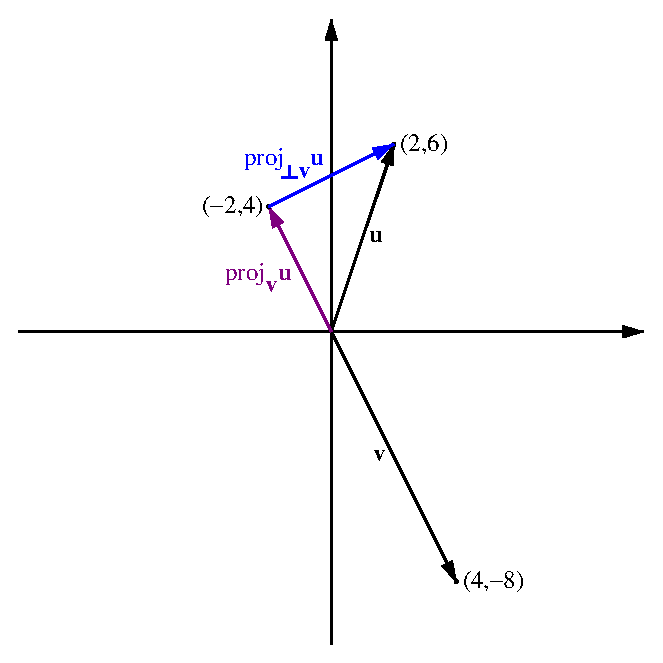
\includegraphics{figures/9_3_Act_4_sol}}
%\caption{Vectors and their projections.}
%\label{F:9.3.Act_4_sol}
\end{center}
%\end{figure}

\end{activitySolution}
\aftera